\section{Sortieralgorithmen}

\begin{frame}[fragile]
\frametitle{Sortieralgorithmen}
Um Binäre Suche anwenden zu können muss unser Array jedoch bereits sortiert sein. Dafür benutzen wir Sortieralgorithmen. Welche kennen sie aus der Vorlesung?
\end{frame}

\begin{frame}[fragile]
\frametitle{Sortieralgorithmen}
Um Binäre Suche anwenden zu können muss unser Array jedoch bereits sortiert sein. Dafür benutzen wir Sortieralgorithmen. Welche kennen sie aus der Vorlesung?
\begin{itemize}
    \item Insertion Sort
    \item Merge Sort
\end{itemize}
\end{frame}

\begin{frame}
\frametitle{Insertion Sort - Funktionsweise}
\begin{enumerate}
    \item Starte mit dem zweiten Element der Liste.
    \item Vergleiche das aktuelle Element mit den Elementen der sortierten Teilliste (links davon).
    \item Füge das aktuelle Element an der richtigen Position in die sortierte Teilliste ein.
    \item Wiederhole die Schritte 2-3 für alle verbleibenden Elemente.
\end{enumerate}
\end{frame}

\begin{frame}[fragile]
\frametitle{Insertion Sort - Beispiel}
\begin{center}
    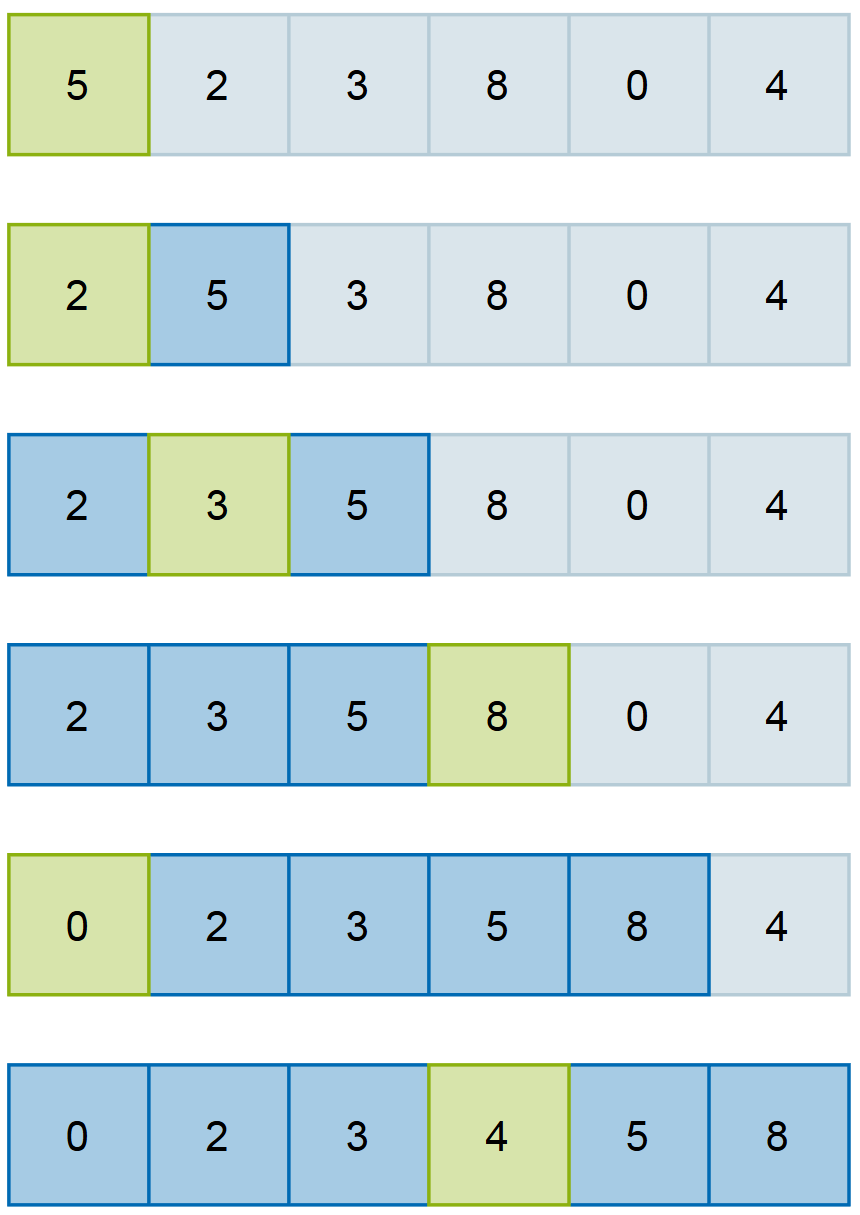
\includegraphics[height=0.75\textheight]{images/insertionSort}
\end{center}
\end{frame}

\begin{frame}[fragile]
\frametitle{Merge Sort - Funktionsweise}
\begin{enumerate}
    \item Teile die Liste rekursiv in zwei Hälften, bis jede Teilliste nur noch ein Element enthält.
    \item Sortiere die Teillisten, indem du sie paarweise vergleichst und zusammenführst.
    \item Wiederhole den Zusammenführungsprozess, bis eine vollständig sortierte Liste entsteht.
\end{enumerate}
\end{frame}

\begin{frame}[fragile]
\frametitle{Merge Sort - Beispiel}
\begin{center}
    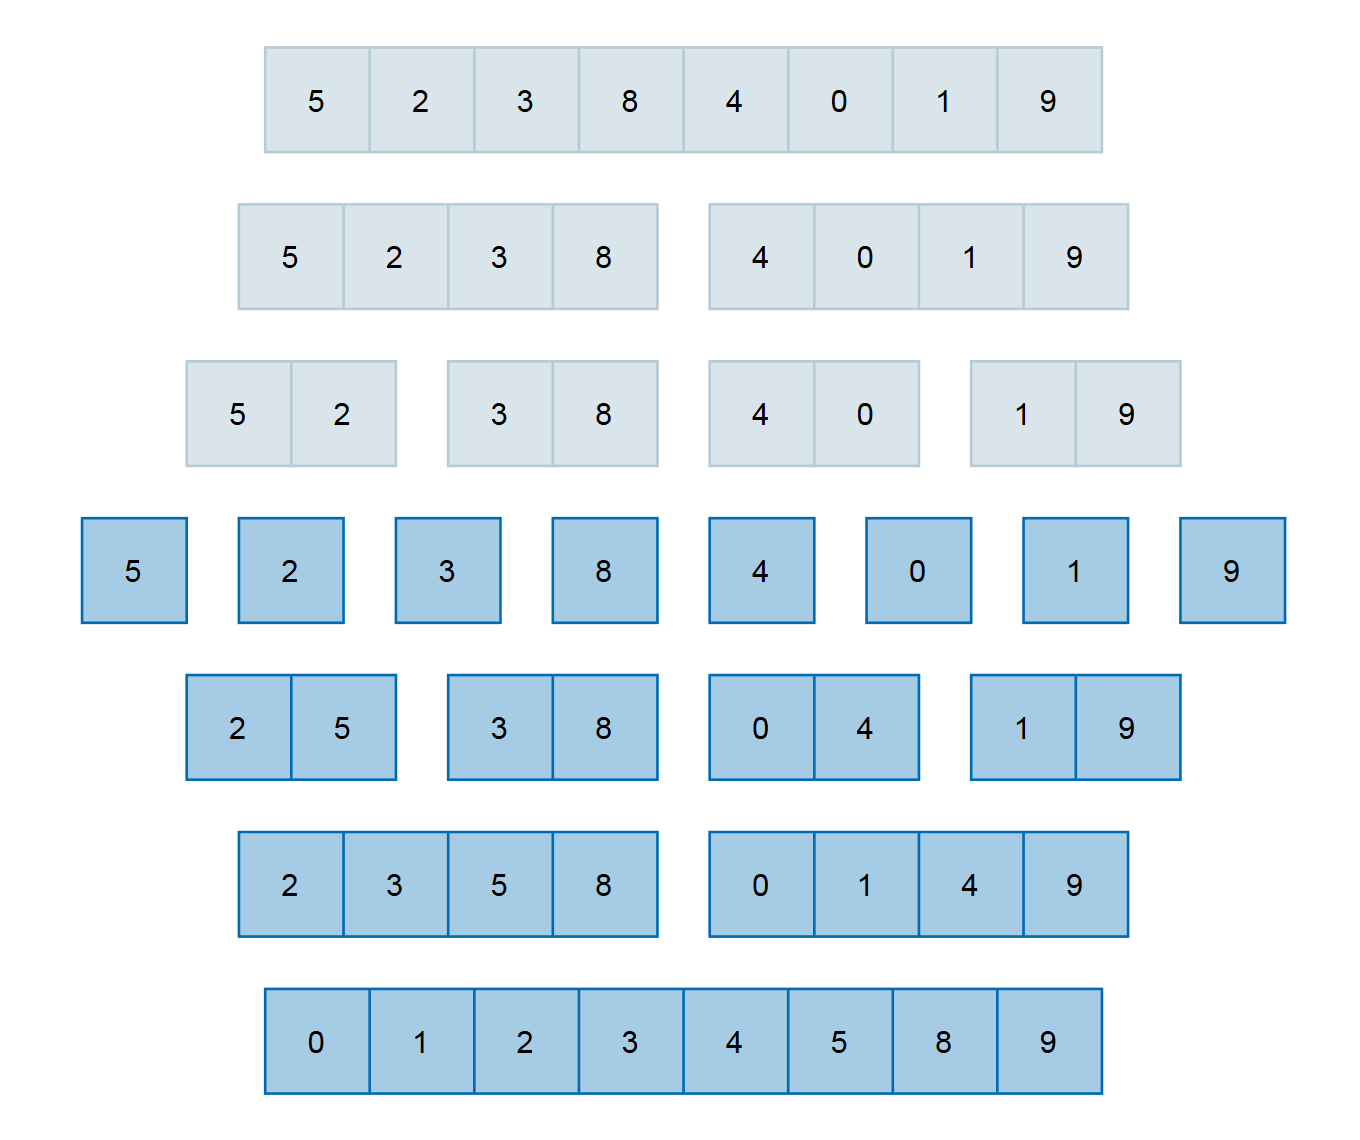
\includegraphics[height=0.75\textheight]{images/mergeSort}
\end{center}
\end{frame}

